%!TEX root = main.tex
\newpage
\section{System}
\subsection{System Architecture}

We have implemented \system\ as a web-based tool on top of a PostgreSQL database. In Figure X we present the system architecture of \system\ , which consists of three core modules: the traversal module, the query module, and the stats module. The traversal module contains several alternative algorithms for traversing the visualization hierarchy. These algorithms are responsible for both generating the visualization hierarchy and identifying the solution (dashboard) from the hierarchy. For generating the visualization hierarchy, the traversal module passes the list of visualizations to be generated to the query module. The query module translates these visualizations into queries, and then optimizes (by grouping) and executes the queries. The stats module is an optional module that allows the traversal module to prune low-utility visualizations without actually generating them. Specifically, it generates coarse statistics for the unexplored visualizations based on the current list of explored visualizations. 

\begin{center}
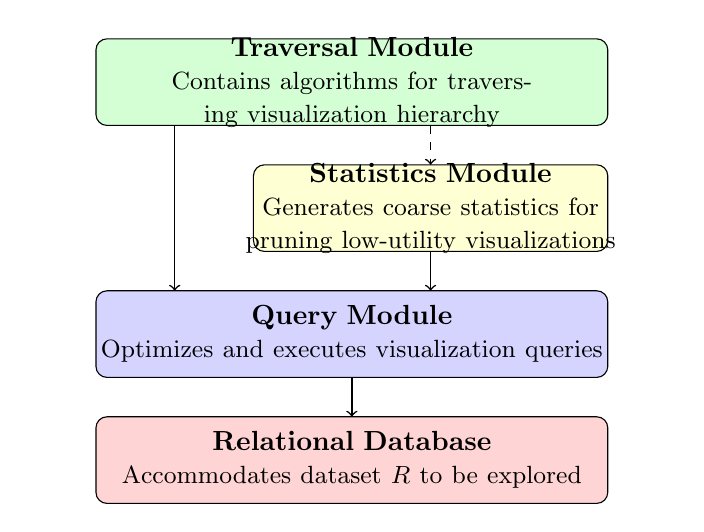
\begin{tikzpicture}
    \filldraw [fill={rgb:red,1;white,5}, rounded corners=4pt] (0, 0) rectangle (6.5, 1.1) node[pos=.5, align=center, text width=8cm] {\textbf{Relational Database}\\ {\small Accommodates dataset $R$ to be explored}};
    \filldraw [fill={rgb:blue,1;white,5}, rounded corners=4pt] (0, 1.6) rectangle (6.5, 2.7) node[pos=.5, align=center, text width=8cm] {\textbf{Query Module}\\ {\small Optimizes and executes visualization queries}};
    \filldraw [fill={rgb:yellow,1;white,5}, rounded corners=4pt] (2, 3.2) rectangle (6.5, 4.3) node[pos=.5, align=center, text width=5cm] {\textbf{Statistics Module}\\ {\small Generates coarse statistics for pruning low-utility visualizations}};
    \filldraw [fill={rgb:green,1;white,5}, rounded corners=4pt] (0, 4.8) rectangle (6.5, 5.9) node[pos=.5, align=center, text width=8cm] {\textbf{Traversal Module}\\ {\small Contains algorithms for traversing visualization hierarchy}};
    \draw [->, line width=0.2mm] (1, 4.8) -- (1, 2.7);
    \draw [->, dashed, line width=0.2mm] (4.25, 4.8) -- (4.25, 4.3);
    \draw [->, line width=0.2mm] (4.25, 3.2) -- (4.25, 2.7);
    \draw [->, line width=0.2mm] (3.25, 1.6) -- (3.25, 1.1);
\end{tikzpicture}
\end{center}

\subsection{Algorithms}
We give an overview of the traversal algorithms to generate the visualization hierarchy and identify visualizations from this hierarchy. We start with offline approach where we first generate the complete hierarchy of visualizations, and then work towards identifying the maximum utility solution. Then, we present our online algorithms to identify a solution in a single phase. 


\subsection{User Interaction}
\begin{figure}[ht!]
\label{overview}
\centering
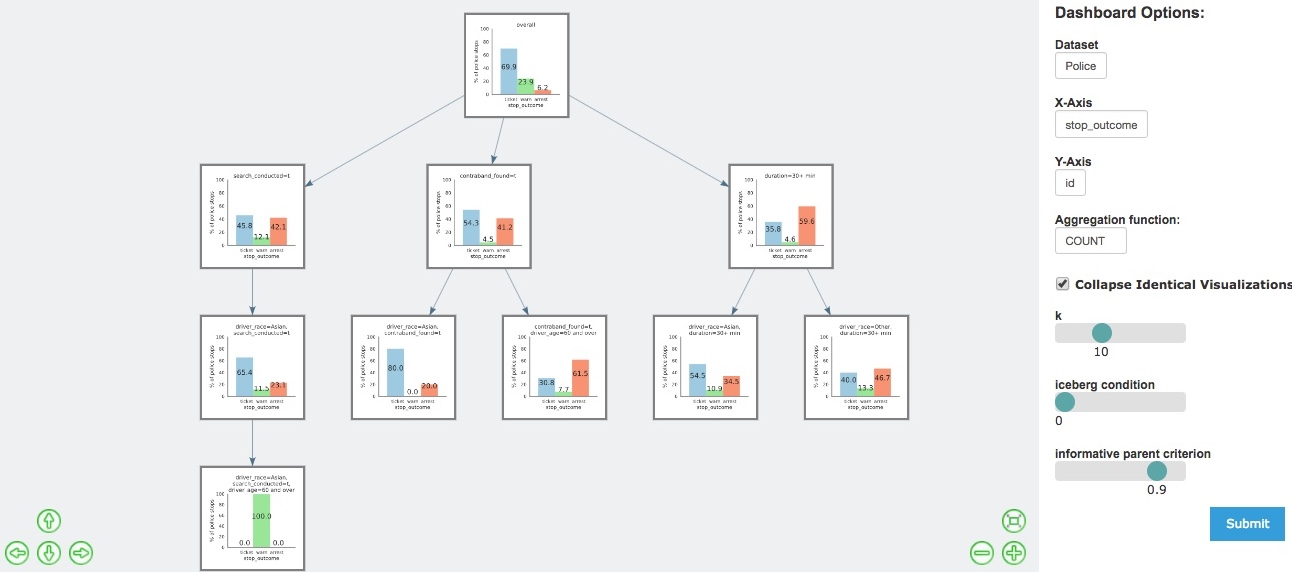
\includegraphics[width=\linewidth]{figures/overview.jpeg}
\caption{Overview of the \system interface for the Police Dataset. Users can select x and y axes of interest, as well as a choice of an aggregation function (COUNT,SUM,AVRG). Default values are set for system related parameters such as the number of visualizations to show in the dashboard (k), iceberg criterion for pruning, and informative parent criterion, which can be adjusted by the users via the sliders if needed.}
\end{figure}
\par Figure \ref{overview} shows an overview of what the \system interface looks like. After the users selects the x and y axes of interest, aggregation function, and optional system parameter settings, an initial dashboard of k visualization is displayed on the canvas. The system provides toolbar buttons with keyboard binding for zooming in, out, and extent, as well as moving around the canvas. Alternatively, participants can also zoom and pan with mouse click and scroll.
\par After browsing through the visualizations the dashboard, users may be interested in getting more information about a particular node. \system supports a mechanism for users to request additional summarizations based on a chosen node of interest. As shown in Figure \ref{altroot_expansion}, the analysts starts with a k=5 visualization. He learns that for the drivers who had contraband found in the vehicle, the arrest rate for drivers who are 60 and over is surprisingly higher than usual, whereas for Asian drivers the arrest rate is lower. Apart from the contraband found stories, he is interested in learning more about the other factor that contribute to high arrest rate: duration=30+min. He clicks on the corresponding visualization and requests for 2 additional visualizations. The system uses the same models and algorithms as discussed earlier to generate the expansion dashboard, with the only difference that the starting node is now the selected visualization, rather than the overall visualization. This node expansion capability is similarly motivated by the idea of \textit{iterative view refinement} in other visual analytics system\cite{Wongsuphasawat2016,Hoque2017}, which is essential for the users to iterate on and explore different hypotheses. 
\begin{figure}[ht!]
\centering
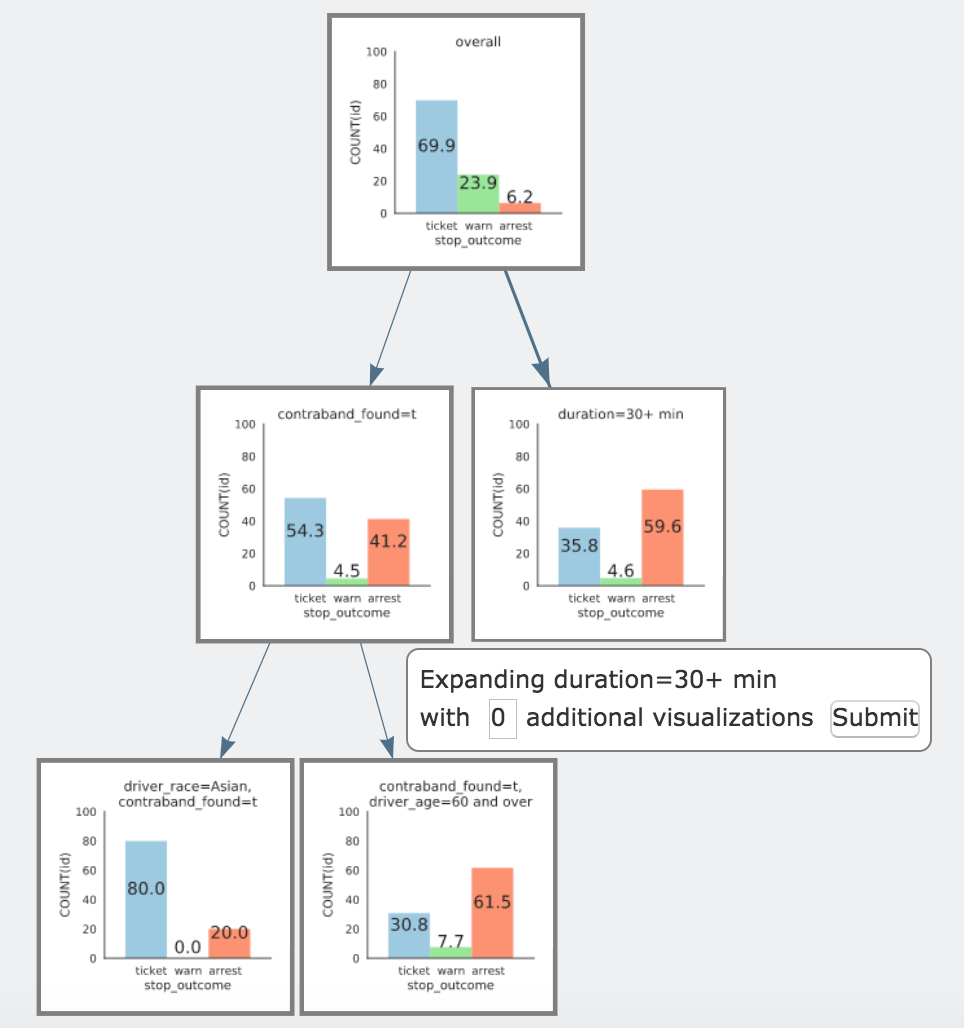
\includegraphics[width=0.43\linewidth]{figures/before_expansion2.png}
\raisebox{5\height}{
\includegraphics[width=0.05\linewidth]{figures/arrow_right.jpeg}}
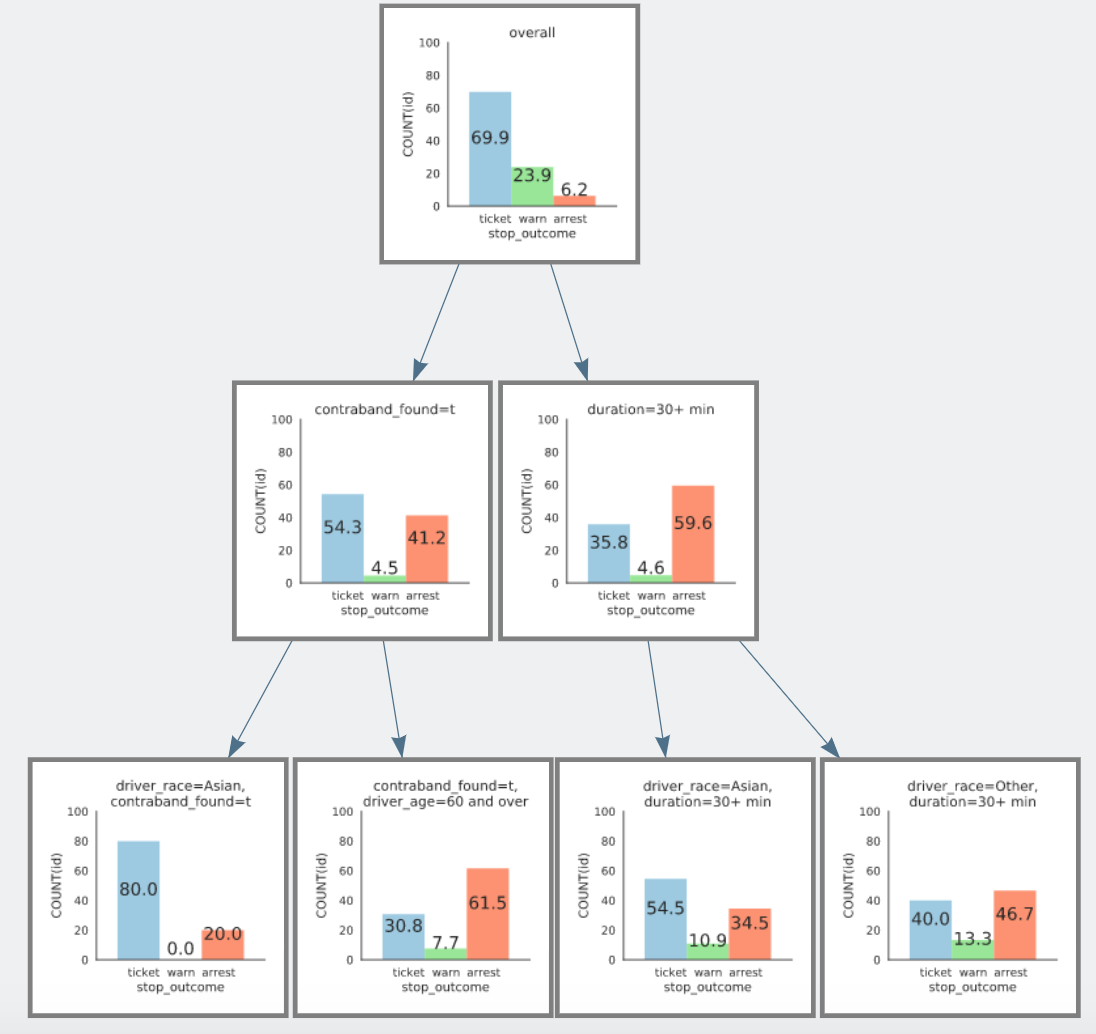
\includegraphics[width=0.49\linewidth]{figures/after_expansion3.png}
\caption{Left: Original k=5 dashboard with the duration=30+min visualization clicked. A pop-up is displayed to submit the request for additional summary visualizations to be generated. Right: Resulting dashboard after requesting for 2 more visualizations based on the visualization of interest.}
\label{altroot_expansion}
\end{figure}
\subsection{Assistive tools for visualizing large lattices}
Due to the amount of space occupied by the hierarchical layout when the number of visualizations gets large, we have developed tools to help users navigate through difference parts of the dashboard interactively. 
\par \textbf{Navigation Minimap:}  When the user zooms in on the dashboard, an overview mini-map is shown on the upper right-hand side of the canvas to help users identify which region of the dashboard they are exploring, as shown in Figure \ref{hover_minimap}. 
\par \textbf{Collapsed visualizations:} 
One observation that we found across several datasets was that many of the visualization attributes resulted in identical distributions. Apart from their attribute name, these visualizations are not very informative for the users, therefore, we offer an option to collapse these visualization, as demonstrated in Figure \ref{collapse_demo}. A visualization can be collapsed if it has more than one redundant sibling and does not have any children. As shown in Figure \ref{hover_minimap}, collapsed nodes can be easily identified by an orange border and the details of which visualizations are in the collapsed node are displayed when the user hovers over the visualization.
\begin{figure}[ht!]
\label{collapse_demo}
\centering
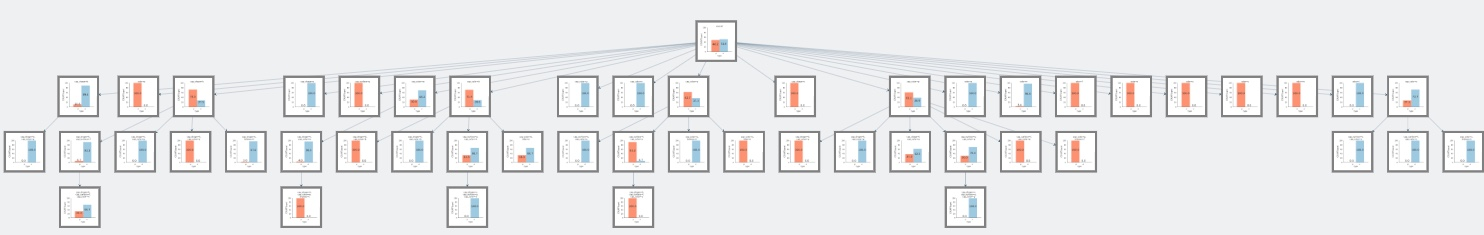
\includegraphics[width=\linewidth]{figures/k50_original.jpeg}
% \noindent\makebox[\linewidth]{\rule{\linewidth}{0.4pt}}
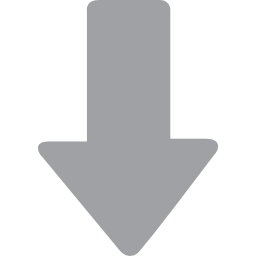
\includegraphics[width=0.05\linewidth]{figures/arrow_down.png}
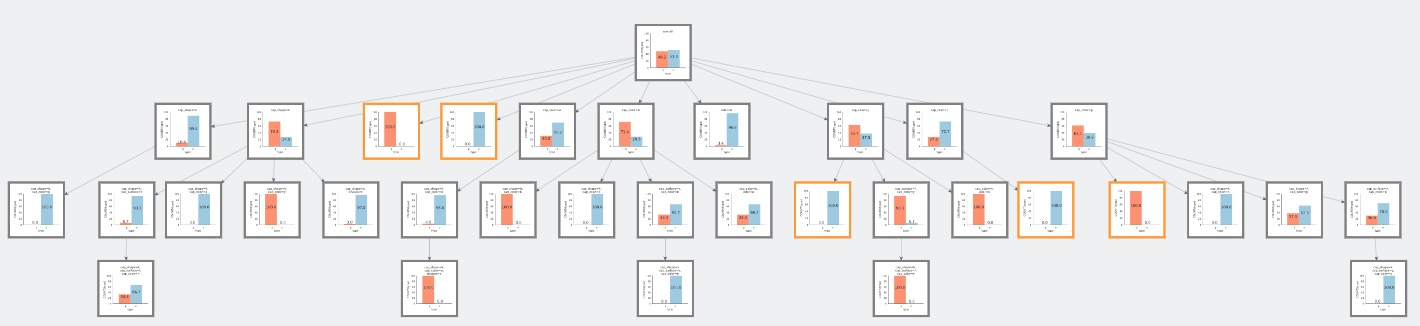
\includegraphics[width=\linewidth]{figures/k50_collapsed.jpeg}
\caption{An example of the k=50 dashboard for the mushroom dataset, which contains type =\{ posionous, edible\} on the x-axis. The collapsed dashboard (bottom) removed 16 redundant visualizations from the original dashboard (top).}
\end{figure}

\begin{figure}[ht!]
\label{hover_minimap}
\centering
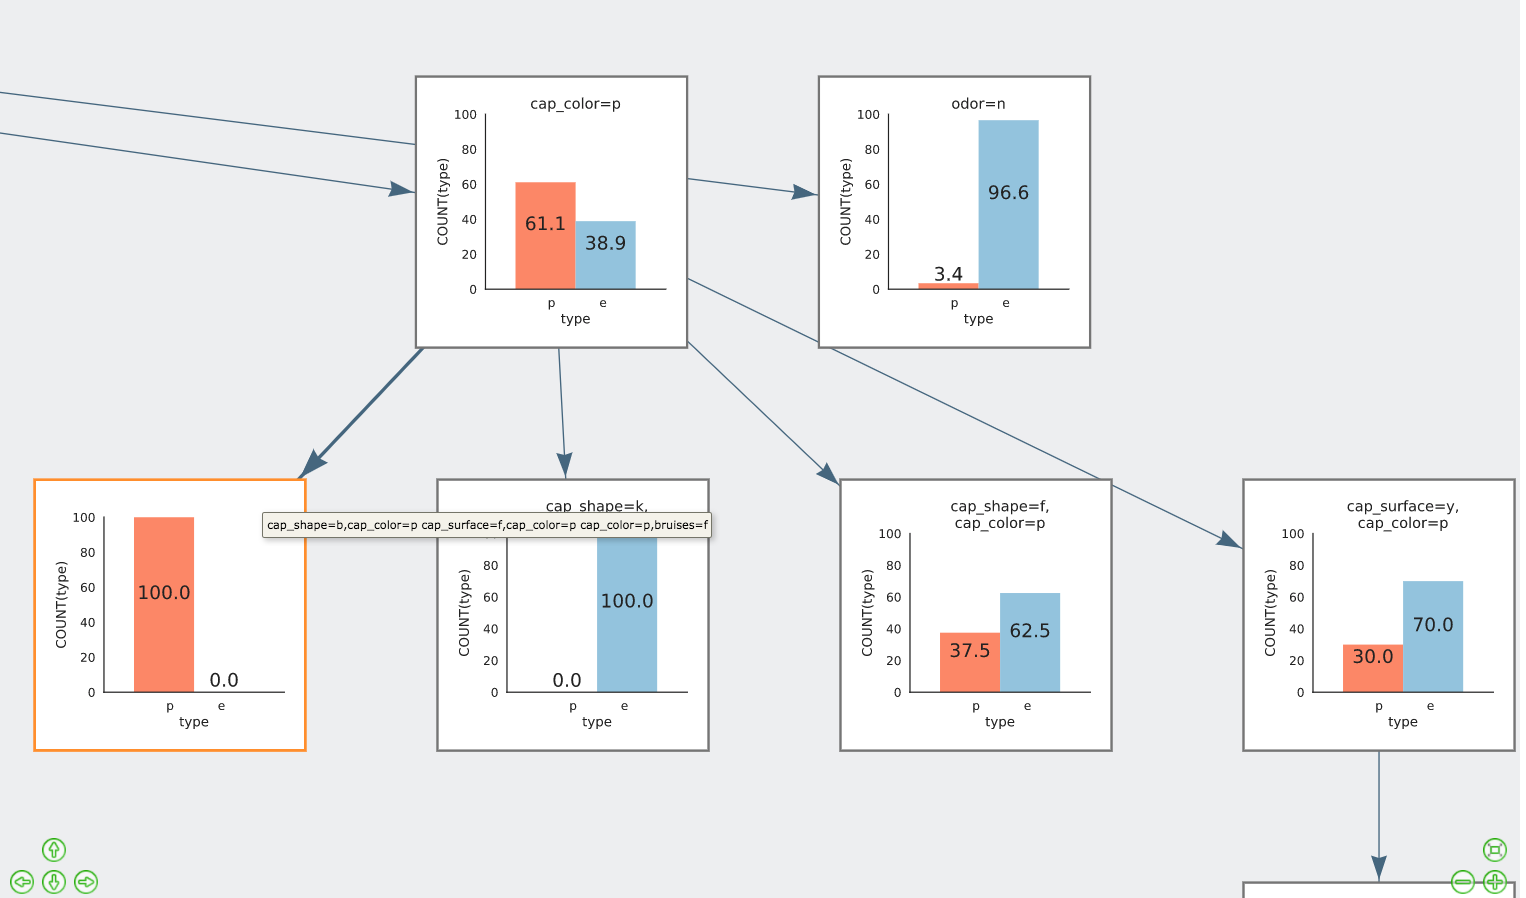
\includegraphics[width=\linewidth]{figures/hoverLabel_minimap.jpg}
\caption{Zoomed-in version of Figure \ref{collapse_demo} showing the labels of a collapsed visualization. The navigation minimap is shown in the top-right to help users navigate through the a large dashboard.}
\end{figure}
